\documentclass{article} % For LaTeX2e
\usepackage{nips15submit_e,times}
\usepackage{hyperref}
\usepackage{url}
\usepackage{lineno}
\usepackage{graphicx}
\usepackage{amsmath}
\usepackage{multicol}
\usepackage[all]{hypcap} 
%\linenumbers% Uncomment for line numbers



\title{America's Warzone: Predicting Gun Violence in Chicago}

\author{
Reuben K. McCreanor\thanks{Department of Statistical Science, Duke University} \\  
\texttt{reuben.mccreanor@duke.edu} \\
\And
Anna Yanchenko\footnotemark[1] \\
\texttt{anna.yanchenko@duke.edu} \\
\And 
Lei Qian\footnotemark[1] \\
\texttt{lei.qian@duke.edu} \\
\And
Megan Robertson\footnotemark[1] \\
\texttt{megan.robertson@duke.edu} \\ 
}

\hypersetup{
    colorlinks=true,
    linkcolor=blue,
    filecolor=magenta,      
    urlcolor=cyan,
    pdftitle={Sharelatex Example},
    bookmarks=true,
    pdfpagemode=FullScreen,
}


\newcommand{\fix}{\marginpar{FIX}}
\newcommand{\new}{\marginpar{NEW}}

\nipsfinalcopy 

\begin{document}

\maketitle

\begin{abstract}
This paper is poop. \newline
\end{abstract}

\section{Introduction}
\label{headings}

\noindent When one thinks of crime in America, Chicago is a city that often comes to mind. Donald Trump frequently discusses the issues of crime in Chicago. According to the Chicago Tribune, there were 4,367 shooting victims in Chicago in 2016. In the same year there were also 785 homicides.\hyperlink{Ref2}{[2]} However, other reports cite that Chicago should not be called the “crime capital” of America. It’s violent rate is less than other cities such as St.  Louis and Detroit. \hyperlink{Ref1}{[1]} This project examines crime in Chicago, specifically armed robberies, from 2011-2017. \newline

\section{Data}
\label{headings}

\noindent The crime data used for this project comes from the City of Chicago’s website. \footnote{Crimes 2001 to present, \url{https://data.cityofchicago.org/Public-Safety/Crimes-2001-to-present/ijzp-q8t2/data}} The data contains every reported crime in Chicago from 2001 to present day. In addition to the type of crime reported (battery, assault, etc.), there is information on the location, time, and other details. The data set was reduced to only armed robberies. 

\begin{figure}[h]
\begin{center}

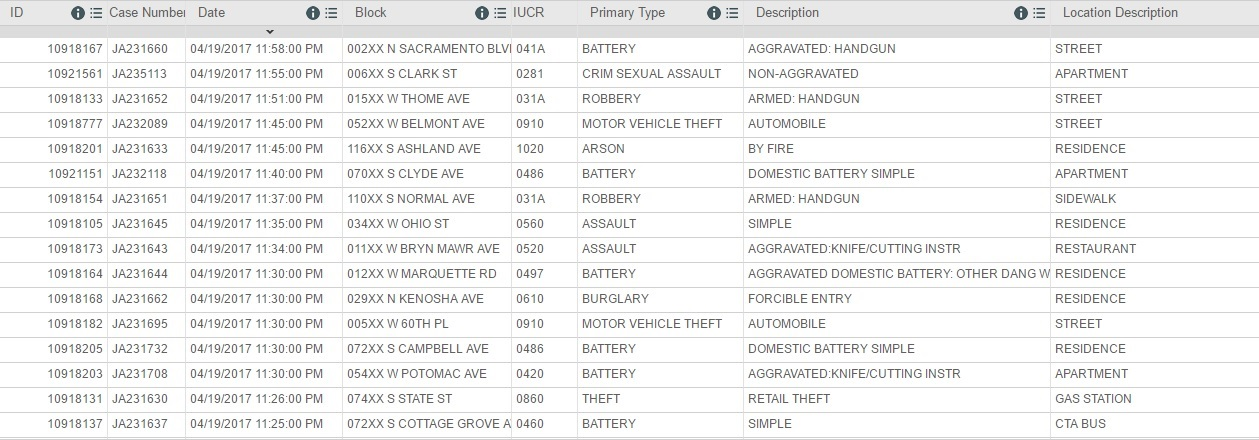
\includegraphics[width=0.8\textwidth,keepaspectratio]{data.jpg}
\caption{The city of Chicago website provides a data set containing information on crimes commited in the city from 2001 to present day.}
\label{data}
\end{center}
\end{figure}

\section{EDA}

\section{Time Series Analysis}

\subsection{Models}

\noindent The city of Chicago is divided into neighborhoods known as sides. These areas can be seen in \autoref{sides}. The borders below are the boundaries of the community area colored by the side.  

\begin{figure}[h]
\begin{center}

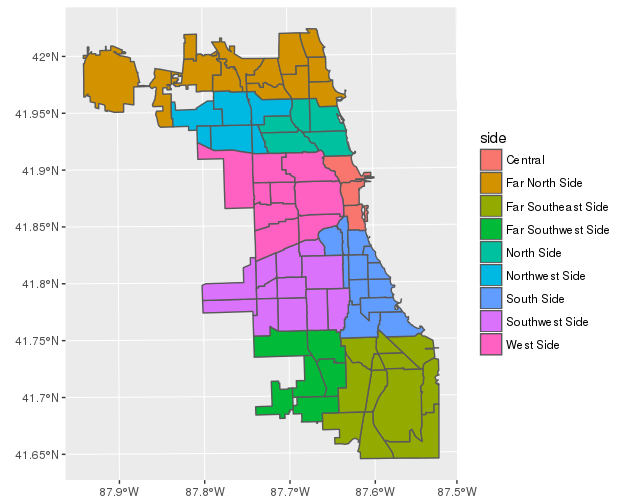
\includegraphics[width=0.8\textwidth,keepaspectratio]{CopyOfside.png}
\caption{The "sides" of Chicago.}
\label{sides}
\end{center}
\end{figure}

\noindent Models were fit to predict the counts of armed robberies in each side between 2003-2016. In order to determine the type of model, the ACF and PACF plots were examined for the data for each of the sides. For example, if there was structure in the PACF plot beyond one lag, moving average terms were added. The model residuals were also examined to ensure there was no remaining structure in the resiudals. 

\begin{multicols}{2}
\begin{figure}[H]
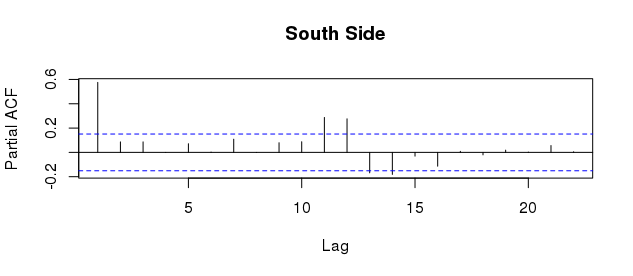
\includegraphics[width = 80mm]{Plots/south_PACF.png}
\end{figure}

\begin{figure}[H]
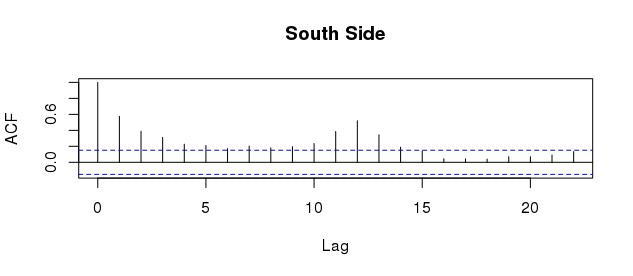
\includegraphics[width=80mm]{Plots/south_ACF.png}
\end{figure}

\end{multicols}

\newpage


\subsubsection*{References}


\hypertarget{Ref1}{[1]} Papachristos, Andrew V., "48 Years of Crime in Chicago: An Analysis of of Serious Crime Trends from 1965-2013,\url{http://isps.yale.edu/sites/default/files/publication/2013/12/48yearsofcrime_final_ispsworkingpaper023.pdf}, December 2013.

\hypertarget{Ref2}{[2]} Pearson, Rick, "Trump Again Assails Chicago gun violence in speech to Congress", \textit{Chicago Tribune}, \url{http://www.chicagotribune.com/news/local/politics/ct-donald-trump-congress-speech-chicago-met-20170228-story.html}, March 2017.


\clearpage
\newpage

\section{Appendix}
\label{headings}


\subsection{Time Series Modeling Plots}
\label{appendix_regression}


\end{document}


